% Options for packages loaded elsewhere
\PassOptionsToPackage{unicode}{hyperref}
\PassOptionsToPackage{hyphens}{url}
\PassOptionsToPackage{dvipsnames,svgnames,x11names}{xcolor}
\documentclass[
]{article}
\usepackage{xcolor}
\usepackage[margin=1in]{geometry}
\usepackage{amsmath,amssymb}
\setcounter{secnumdepth}{-\maxdimen} % remove section numbering
\usepackage{iftex}
\ifPDFTeX
  \usepackage[T1]{fontenc}
  \usepackage[utf8]{inputenc}
  \usepackage{textcomp} % provide euro and other symbols
\else % if luatex or xetex
  \usepackage{unicode-math} % this also loads fontspec
  \defaultfontfeatures{Scale=MatchLowercase}
  \defaultfontfeatures[\rmfamily]{Ligatures=TeX,Scale=1}
\fi
\usepackage{lmodern}
\ifPDFTeX\else
  % xetex/luatex font selection
\fi
% Use upquote if available, for straight quotes in verbatim environments
\IfFileExists{upquote.sty}{\usepackage{upquote}}{}
\IfFileExists{microtype.sty}{% use microtype if available
  \usepackage[]{microtype}
  \UseMicrotypeSet[protrusion]{basicmath} % disable protrusion for tt fonts
}{}
\makeatletter
\@ifundefined{KOMAClassName}{% if non-KOMA class
  \IfFileExists{parskip.sty}{%
    \usepackage{parskip}
  }{% else
    \setlength{\parindent}{0pt}
    \setlength{\parskip}{6pt plus 2pt minus 1pt}}
}{% if KOMA class
  \KOMAoptions{parskip=half}}
\makeatother
\usepackage{longtable,booktabs,array}
\usepackage{caption}
\captionsetup[table]{skip=6pt}
\newcounter{none} % for unnumbered tables
\usepackage{calc} % for calculating minipage widths
% Correct order of tables after \paragraph or \subparagraph
\usepackage{etoolbox}
\makeatletter
\patchcmd\longtable{\par}{\if@noskipsec\mbox{}\fi\par}{}{}
\makeatother
% Allow footnotes in longtable head/foot
\IfFileExists{footnotehyper.sty}{\usepackage{footnotehyper}}{\usepackage{footnote}}
\makesavenoteenv{longtable}
\usepackage{graphicx}
\makeatletter
\newsavebox\pandoc@box
\newcommand*\pandocbounded[1]{% scales image to fit in text height/width
  \sbox\pandoc@box{#1}%
  \Gscale@div\@tempa{\textheight}{\dimexpr\ht\pandoc@box+\dp\pandoc@box\relax}%
  \Gscale@div\@tempb{\linewidth}{\wd\pandoc@box}%
  \ifdim\@tempb\p@<\@tempa\p@\let\@tempa\@tempb\fi% select the smaller of both
  \ifdim\@tempa\p@<\p@\scalebox{\@tempa}{\usebox\pandoc@box}%
  \else\usebox{\pandoc@box}%
  \fi%
}
% Set default figure placement to htbp
\def\fps@figure{htbp}
\makeatother
\setlength{\emergencystretch}{3em} % prevent overfull lines
\providecommand{\tightlist}{%
  \setlength{\itemsep}{0pt}\setlength{\parskip}{0pt}}
\usepackage{bookmark}
\IfFileExists{xurl.sty}{\usepackage{xurl}}{} % add URL line breaks if available
\urlstyle{same}
% fallback for those not using the hyperref driver hyperxmp:
\makeatletter
\@ifundefined{xmpquote}{\newcommand{\xmpquote}[1]{#1}}{}
\makeatother
\hypersetup{
  pdftitle={The Persistence Boundary: A Measurable Spectral Law for the Whitening Knee in Muon-style Optimization},
  colorlinks=true,
  linkcolor={blue},
  filecolor={Maroon},
  citecolor={Blue},
  urlcolor={blue},
  pdfcreator={LaTeX via pandoc}}

\title{The Persistence Boundary: A Measurable Spectral Law for the
Whitening Knee in Muon-style Optimization}
\author{}
\date{Working draft v3 --- 2026-08-25}

\begin{document}
\maketitle

\textbf{Status: working draft v3 (2026-08-25). All numbers measured in
this repository; probe IDs refer to \texttt{research\_runs/probe\_*}
logs and \texttt{research/OPTIMIZER\_RESEARCH.md} §0.5. Figures render
from raw logs via \texttt{experiments/paper\_figs.py} (no manual
plotting).}

\begin{quote}
\textbf{v2 \(\to\) v3: the tracked gaps are closed.} 1. The U-curve is
now single-frame: classic / cubic5 / b10 were re-run post-fix
(P31--P33); the five-point U lives entirely in the current frame (§5.2).
2. Both arms and the peak now have 3 seeds each (P25, P36--P39); every
arm-vs-peak difference is positive on every seed (§5.2, §6). 3. Dense
platform: the knee grid is now 5 points (b002/b005/b01/b05/b10; P34/P35
added) \textbf{plus a 2000-step paired tier (P40--P42) that reverses the
500-step dense ranking} --- the 500-step winner b002 destabilizes (spike
at step \(\approx\){}600, NaN by \(\approx\){}1000, paired control
clean on identical data) and b005 concedes +0.072 to b05. Warmup knee
optima bias downward; the steady-state optimum sits at the band's upper
edge on both architectures (§5.4). The MoE-side 2000-step knee check
(P43 b10 vs.~P28a b05) shows the mirror asymmetry: b10's +0.08 warmup
penalty closes to -0.02 by step 1900 --- under-whitening fades,
injection compounds; the b05 default now rests on 2000-step evidence. 4.
The transition-band upper edge has an operational definition --- first
log-\(\sigma\) bin whose excess persistence (median \(\rho\) - median
floor) reaches \(\geq\) 0.9 --- and all \(\sigma^*_{\mathrm{upper}}\)
values are recomputed under it (\texttt{experiments/sigma\_upper*.py};
§4.3). 5. §7's per-head row is ``consistent, not confirmed'' (softened;
the pre-fix harm did not reproduce post-fix).

\textbf{Correction in v3.} The §4.1 KS statistic against an MP bulk for
the 768\(\times\){}768 group was numerically invalid (uniform-grid CDF
integration diverges under the c = 1 MP density singularity at y = 0; on
synthetic pure-MP data the same code reports D \(\approx\) 0.60). The
rejection of MP calibration rests on the remaining, unaffected evidence
(§4.1).
\end{quote}

\section{Abstract}\label{abstract}

Muon-style optimizers orthogonalize the momentum matrix with
Newton--Schulz (NS) iterations whose scalar spectral response is a
design choice. Recent relaxed schedules leave a \emph{knee}: singular
values below a threshold receive near-zero weight instead of being
flattened to 1 --- and are both cheaper and better. But where should the
knee sit? We turn this hyperparameter question into a measurement
question. First, we show the natural closed-form answer from
random-matrix theory (knee = Marchenko--Pastur bulk edge \(\lambda_+\))
fails on real training momentum: spectra are smooth heavy-tailed (Zipf
slopes -0.7\ldots-2.7), entry noise is anisotropic at ratios of
10\(^2\)--10\(^4\), and spike peeling diverges. Second, we show the
question can still be answered assumption-free: cross-microbatch
direction persistence \(\rho(\sigma)\) collapses sharply at a measurable
boundary \(\sigma^*\), stationary across our training window
(micro-steps 300\(\to\){}1900). Third, we state and validate the
resulting law: \(\sigma^*\) is the \emph{lower} edge of a transition
band whose persistent-signal fraction climbs from \(\approx\){}0.3 to
\(\approx\){}1; the quality-optimal knee sits at the band's
\emph{upper} edge, and the two arms of the U-shaped quality curve are
exactly the band's width (+0.05 nat when the knee is at the lower edge;
+0.09 when past the upper edge). The law replicates across architectures
--- with a horizon twist. On a 132M dense model \(\sigma^*\) is
\textasciitilde10\(\times\) lower than on a 1080M MoE, and the
warmup-tier optimum moves with it (five-point grid); but by 2000 steps
the dense ranking reverses --- the lowest knee destabilizes (NaN after a
step-600 spike), the mid-band point concedes 0.07 nat, and the shared
steady-state optimum sits at the band's upper edge (knee50 \(\approx\)
0.01) on \emph{both} architectures. The asymmetry is structural:
under-whitening is paid upfront, variance injection compounds. A method
built on the naive binary rule (per-shape knees at \(\sigma^*\),
``EdgeCubic'') is neutral at 500 steps but degrades monotonically by
2000 steps (+0.47 nat on the auxiliary MTP loss), with the damage
localized in exactly the group the corrected law flags --- a controlled
negative result that doubles as the law's stress test. Six previously
reported failure modes of spectral shaping, plus Pion's RLVR
observation, admit a single zero-parameter account. Practically: the
knee is not a constant to tune but a boundary to measure --- and in our
stack the measured optimum coincides with the existing cubic5b05
schedule, which we retain as default.

\section{1. Introduction}\label{introduction}

The Muon family replaces the update direction for a 2D weight matrix by
an orthogonalization of its momentum M =
U\(\Sigma\){}V\(^{\mathsf{T}}\). The polar factor UV\(^{\mathsf{T}}\)
is never computed exactly: a fixed Newton--Schulz polynomial iteration
reshapes the singular values through a scalar response \(\tau(\sigma)\).
``How Much Orthogonalization Does Muon Need?'' (arXiv 2606.00371) showed
that training quality is \emph{not} monotone in the accuracy of this
map: a relaxed-cubic schedule with a pronounced knee (small \(\sigma\)
lifted only to \(\approx\){}0.12 instead of \(\approx\){}1) is both
cheaper and better. Pion (arXiv 2605.19282) independently found that
suppressing the small-\(\sigma\) tail helps in low-SNR regimes (RLVR,
VLA). Neither work says where the knee \emph{should} sit; both inherit
it from numerical considerations (bf16 resolution).

This paper answers ``where is the knee'' with a law that is:

\begin{itemize}
\tightlist
\item
  \textbf{Measurable.} The boundary \(\sigma^*\) is read directly off
  cross-microbatch gradient correlations, with no distributional
  assumption (§2.3, §4).
\item
  \textbf{Stationary.} \(\sigma^*\) does not drift over the probed
  training window (micro-steps 300--1900; §4.3).
\item
  \textbf{Intervention-validated.} Quality vs.~knee position is
  U-shaped, and the U's arms coincide with the measured \emph{transition
  band} {[}\(\sigma^*\), \(\sigma^*_{\mathrm{upper}}\){]}: knees at the
  lower edge over-inject non-persistent directions, knees past the upper
  edge under-whiten persistent ones (§5).
\item
  \textbf{Cross-architecture.} On a 132M dense model \(\sigma^*\) is
  \(\approx\){}10\(\times\) lower than on a 1080M MoE, and the
  empirically optimal knee moves by the same factor --- the law
  replicates as ``optimum = measured band'', not as a universal constant
  (§5.4).
\item
  \textbf{Unifying.} Six in-house failure/quality results and one
  literature observation (Pion on RLVR) follow from one mechanism with
  zero fitted parameters (§7).
\end{itemize}

We also report the theory that motivated the measurement --- an
equivariance classification of update rules and a closed-form
shrink-then-whiten optimum \(t^*(\sigma)\) under a spiked model (§3) ---
and \emph{where it breaks}: real momentum is neither spiked nor
isotropic, so the closed form calibrates incorrectly while its shape
intuition survives (§4.1). A deliberate method attempt built on the
naive reading of the law (``EdgeCubic'', per-shape knees at
\(\sigma^*\)) fails at longer horizons in exactly the way the corrected
law predicts (§8). We count this as evidence: the law is falsifiable in
both directions, and it called the failure's location in advance.

\textbf{Contributions.}

\begin{enumerate}
\def\labelenumi{\arabic{enumi}.}
\tightlist
\item
  A snapshot-and-persistence measurement protocol (momentum +
  micro-batch gradients \(\to\) \(\rho(\sigma)\) \(\to\) per-shape-group
  \(\sigma^*\)), with the analysis chain validated on synthetic
  spiked-MP ground truth (\(\hat{\lambda}_+\) within 2\%, spike \(\rho\)
  0.91 vs. BGN-theoretical 0.87--0.96).
\item
  The persistence-boundary law for the whitening knee --- including the
  transition-band refinement and its U-curve signature --- validated by
  intervention on two architectures.
\item
  A zero-parameter unified account of six failure modes plus one
  literature observation.
\item
  A controlled negative result (EdgeCubic at 2000 steps) with
  single-variable attribution, doubling as the law's stress test.
\item
  Practical guidance: what to measure before touching the knee; why
  500-step promotion gates are unsafe; why cubic5b05 is already
  near-optimal in our regime.
\end{enumerate}

\section{2. Background and setup}\label{background-and-setup}

\subsection{2.1 Spectral shaping in Muon-style
optimizers}\label{spectral-shaping-in-muon-style-optimizers}

For a 2D weight matrix with momentum M (EMA + nesterov), Muon steps
along Orth(M) \(\approx\) NS(M). Every published variant is a spectral
map --- singular vectors kept, spectrum reshaped by a scalar response:

{\def\LTcaptype{none} % do not increment counter
\begin{longtable}[]{@{}
  >{\raggedright\arraybackslash}p{(\linewidth - 6\tabcolsep) * \real{0.2500}}
  >{\raggedright\arraybackslash}p{(\linewidth - 6\tabcolsep) * \real{0.2500}}
  >{\raggedright\arraybackslash}p{(\linewidth - 6\tabcolsep) * \real{0.2500}}
  >{\raggedright\arraybackslash}p{(\linewidth - 6\tabcolsep) * \real{0.2500}}@{}}
\toprule\noalign{}
\begin{minipage}[b]{\linewidth}\raggedright
variant
\end{minipage} & \begin{minipage}[b]{\linewidth}\raggedright
response
\end{minipage} & \begin{minipage}[b]{\linewidth}\raggedright
GEMMs/matrix
\end{minipage} & \begin{minipage}[b]{\linewidth}\raggedright
knee50
\end{minipage} \\
\midrule\noalign{}
\endhead
\bottomrule\noalign{}
\endlastfoot
classic NS5 (quintic, 5 steps) & band {[}0.65, 1.20{]},
\(\tau\)(1e-3)=0.47 & 15 & \(\approx\){}0.001 \\
Polar Express (PE5) & band {[}0.80, 1.13{]}, \(\tau\)(1e-3)=0.86 & 15 &
\(\lesssim\){}0.001 \\
cubic5 (relaxed, arXiv 2606.00371) & band {[}0.7, 1.3{]},
\(\tau\)(1e-3)=0.12 & 10 & \(\approx\){}0.004 \\
\textbf{cubic5b05 (our default)} & same generator, l0=0.05 & 10 &
\(\approx\){}0.010 \\
cubic5b10 / b002 & l0=0.1 / l0=0.002 (7 steps) & 10 / 14 &
\(\approx\){}0.02 / \(\approx\){}5e-4 \\
\end{longtable}
}

knee50 := the F-normalized singular value receiving half weight,
measured numerically from each schedule's scalar response (it tracks the
design lower-clamp l0 sub-linearly and is the variable we intervene on).
Our optimizer (``MuonH'') additionally projects each updated matrix back
to its pre-update Frobenius norm (hyperball pinning); this detail
interacts with one bug the measurement uncovered (§4.4).

\subsection{2.2 Experimental platforms and noise
discipline}\label{experimental-platforms-and-noise-discipline}

\begin{itemize}
\tightlist
\item
  \textbf{MoE probe platform}: 1080M params --- hidden 768, 8 layers + 1
  MTP block (depth 1), 8 heads, 256 routed experts top-8 + 2 shared
  (intermediate 384), KDA linear-attention layers interleaved; sequence
  1024 with document packing, micro-batch 12 \(\times\) accumulation 2
  (24,576 tokens per optimizer step); formula-derived lr (adam 1.545e-3,
  muon 6.695e-3), warmup 279 micro-steps; bf16, mx.compile, Apple M4
  Max.
\item
  \textbf{Dense platform} (externalization): 132M params --- hidden 768,
  12 layers, 12 heads, dense FFN 3072, no MTP/latent path.
\item
  \textbf{Tiers}: screening = 500 micro-steps (\(\approx\){}14 min);
  confirmation = 2000 micro-steps (\(\approx\){}45 min). Every quality
  claim is a same-seed (1337), same-data-order \textbf{paired}
  comparison. Paired noise floor: \(\pm\){}0.05 nat (Metal
  nondeterminism only). Cross-seed floor: \(\sigma\) = 0.11 nat (3
  seeds: 5.264 / 5.094 / 5.302, P25). Each claim below states which
  floor applies.
\item
  \textbf{Snapshot tooling} (\texttt{trainer/snapshot.py}; env-gated,
  zero overhead when off): at chosen optimizer steps, dump the momentum
  fed into NS and the 2\(\times\){}accum independent micro-batch
  gradients forming consecutive updates, with structured subsampling for
  stacked expert tensors. Analysis: \texttt{experiments/mp\_fit.py}.
\end{itemize}

\subsection{\texorpdfstring{2.3 The measurement: direction persistence
\(\rho(\sigma)\)}{2.3 The measurement: direction persistence \textbackslash rho(\textbackslash sigma)}}\label{the-measurement-direction-persistence-rhosigma}

Split the gradients of two consecutive optimizer updates into their
constituent micro-batches (after accumulation rescaling). For each
F-normalized momentum matrix, take its singular directions
\{\(u_i v_i^{\mathsf{T}}\)\} at a snapshot step and measure how much of
the \emph{subsequent} micro-batch gradient energy aligns with direction
i, in excess of a chance-level floor estimated from the same
micro-batches; bin by \(\sigma\). Persistent directions --- signal, by
definition: the gradient keeps returning to them --- have \(\rho\)
\(\approx\) 1; fresh-noise directions have \(\rho\) \(\approx\) 0. The
boundary \(\sigma^*\) is the collapse point of \(\rho(\sigma)\).

The estimator is validated end-to-end on synthetic spiked-MP ground
truth: bulk \(\rho\) \(\approx\) 0, spike \(\rho\) = 0.91 against the
BGN-theoretical 0.87--0.96, and the recovered bulk edge
\(\hat{\lambda}_+\) within 2\% of truth. Nothing in the estimator
assumes MP, spikes, or isotropy --- which §4 shows is essential.

\section{3. Theory: the search space, the null model, and the
closed-form
optimum}\label{theory-the-search-space-the-null-model-and-the-closed-form-optimum}

This section compresses \texttt{research/SPECTRAL\_THEORY.md} §1--§3,
keeping what the experiments later confirm or refute. Readers who want
only the empirical law can jump to §4.

\subsection{3.1 Classification: equivariant stateless rules are joint
spectral
maps}\label{classification-equivariant-stateless-rules-are-joint-spectral-maps}

Let \(\Phi\): \(\mathbb{R}^{m\times n}\) \(\to\)
\(\mathbb{R}^{m\times n}\) act on momentum. If \(\Phi\) is
\textbf{equivariant} (\(\Phi\)(QMR) =
Q\(\cdot\)\(\Phi\)(M)\(\cdot\){}R for all orthogonal Q, R) and
\textbf{stateless} (depends only on the current M), then by
von-Neumann-type representation theorems \(\Phi\) is a joint spectral
map: \(\Phi\)(M) =
U\(\cdot\){}diag(\(\tau\))\(\cdot\){}V\(^{\mathsf{T}}\) with
\(\tau\) a function of the spectrum. Every published variant (classic
NS5, Polar Express, the cubic family, Pion, fractional-power iterations)
lives in this space; the literature restricts itself to \emph{separable
polynomial} maps \(\tau_i\) = p(\(\sigma_i\)), a proper subset ---
joint, spectrum-adaptive maps are equally legal. Leaving the space
requires one of three channels: breaking equivariance (row statistics
--- NorMuon, RowFloor, Aurora, per-head), adding state (second moments,
SOAP bases, error feedback), or adding curvature (Mousse). This paper
stays inside and asks: what is the optimal \(\tau\)?

\subsection{3.2 Null model: momentum = persistent signal + fresh
isotropic
noise}\label{null-model-momentum-persistent-signal-fresh-isotropic-noise}

Model the F-normalized momentum as X = S + E: S low-rank and persistent,
E i.i.d. entry noise with variance w/(mn) (w = noise fraction of
Frobenius energy). EMA with decay \(\beta\) averages noise down by the
effective sample size ESS = (1+\(\beta\))/(1-\(\beta\)) (39 at
\(\beta\)=0.95) while signal stacks coherently. Random-matrix theory
(Marchenko--Pastur; BBP; Benaych-Georges--Nadakuditi) then gives: a
noise bulk with upper edge \textbf{\(\lambda_+\) =
\(\sqrt{w}\)\(\cdot\)(1/\(\sqrt{m}\) + 1/\(\sqrt{n}\))}; directions
below the edge asymptotically orthogonal to signal; closed-form cosine
overlaps above it. A toy EMA model confirms the machinery end to end:
predicted vs.~measured noise level ratio 0.997; overlap collapse at the
predicted edge (0.757 measured vs.~0.760 theory at \(\sigma\)/edge =
1.27; 0.10 at \(\sigma\)/edge = 0.98).

\subsection{3.3 The in-space optimum:
shrink-then-whiten}\label{the-in-space-optimum-shrink-then-whiten}

The Muon ideal is the polar factor of the \emph{signal} --- whiten all
true descent directions equally. Acting only along observed directions,
both least-squares projection onto the signal polar factor and matched
filtering give the same shape: \(\tau_i\) =
\(\cos\theta_u\)(\(\sigma_i\))\(\cdot\)\(\cos\theta_v\)(\(\sigma_i\)).
Hence the closed form \textbf{\(t^*(\sigma)\)}: zero below
\(\lambda_+\); partial weight just above it (a direction that is mostly
noise gets exactly its overlap fraction); \(\to\){}1 for \(\sigma\)
\(\gg\) \(\lambda_+\).

Three properties. (i) \textbf{Shape}: a knee plus a flat band, with knee
position and transition profile fixed by (m, n, w) --- no
hyperparameter. (ii) \textbf{Legitimacy}: \(t^*\) is monotone and
bounded, hence realizable as the regularized linear-maximization
solution of a convex spectral penalty (a hard knee + flat band is
exactly ``spectral-norm ball \(\cap\) nuclear-norm penalty''), so a
mirror-descent geometry exists and standard convergence theory applies
--- it is not a heuristic. (iii) \textbf{Relation to Gavish--Donoho}: GD
shrinkage reconstructs the signal matrix (\(\tau_{\mathrm{GD}}\) =
\(\hat{s}\)\(\cdot\)\(\cos\theta_u\)\(\cdot\)\(\cos\theta_v\)); our
target is the \emph{whitened} signal (drop \(\hat{s}\)). To our
knowledge this ``optimal shrinkage under a whitening objective'' is
absent from both the RMT and the Muon literature.

\textbf{Compatibility with the impossibility theorem.} Muon-p (arXiv
2606.13867) rules out fixed univariate polynomial iterations converging
to fractional powers \(\sigma^p\). \(t^*\) is unaffected: it tends to a
constant at large \(\sigma\) --- precisely the natural attractor of
NS-type iterations. In this reading the cubic family is a coarse
composite realization of a knee map whose knee is placed by numerics
rather than by statistics.

\subsection{3.4 Where the mathematics allows
cheapness}\label{where-the-mathematics-allows-cheapness}

The cost breakpoint is knee sharpness (Bernstein-ellipse argument). A
single-shot polynomial approximating a knee at \(\ell\) needs degree
\textasciitilde1/\(\sqrt{\text{smoothing radius}}\): measured, a
smoothed \(t^*\) with knee at 0.029 still has 0.33 error and 0.32 noise
leakage at deg-8 (10 GEMMs). Iterated composition grows effective degree
exponentially (k cubic steps \(\equiv\) degree \(3^k\)), cost
\textasciitilde log(1/\(\ell\)). The cubic iteration machinery is
therefore the right substrate; the theory re-prices only its l0 constant
--- and higher knees need \emph{fewer} steps (l0 = 0.03--0.09
\(\Rightarrow\) 3--4 steps, 6--8 GEMMs vs.~10). Cost and quality point
the same way, \emph{if} the knee is placed correctly. §8 tests exactly
this.

\section{4. Measurement: real momentum and the persistence
boundary}\label{measurement-real-momentum-and-the-persistence-boundary}

\subsection{4.1 The closed form fails on real momentum --- and
why}\label{the-closed-form-fails-on-real-momentum-and-why}

Running the snapshot pipeline on the MoE platform (probe\_p18\_snap,
optimizer steps 150/300; both time points agree) kills the spiked-MP
calibration on all three of its assumptions:

\begin{itemize}
\tightlist
\item
  \textbf{Spike peeling diverges} (\(\hat{w}\) \(\to\) 0) for almost
  every shape group. (An earlier draft cited a KS D = 0.60 against an MP
  bulk for the one nominally fittable group, 768\(\times\){}768; that
  statistic was numerically invalid --- uniform-grid CDF integration
  diverges under the c = 1 MP density singularity at y = 0, reporting D
  \(\approx\) 0.60 even on synthetic pure-MP data. The peeling
  divergence stands on its own.)
\item
  \textbf{Spectra are smooth heavy-tailed} --- Zipf slopes
  -0.7\ldots-2.7 in log \(\sigma\)--log rank, no plateau bulk, no
  low-rank spike structure.
\item
  \textbf{Entry noise is strongly anisotropic} --- centered-residual
  row/column variance ratios of 10\(^2\)--10\(^4\) (rows up to 3.2e4,
  columns up to 2.6e4), violating the i.i.d. premise behind
  \(\lambda_+\) = \(\sqrt{w}\)(1/\(\sqrt{m}\) + 1/\(\sqrt{n}\)).
\end{itemize}

Both failure branches flagged in advance in the theory note (anisotropy;
non-spiked signal) are the ones reality takes. The closed form therefore
cannot \emph{place} the knee. What survives is \(t^*\)'s shape logic:
weight each direction by how much of it is signal --- which is exactly
what \(\rho(\sigma)\) measures, without a model.

\subsection{\texorpdfstring{4.2 \(\rho(\sigma)\) collapses sharply: the
boundary \(\sigma^*\)
exists}{4.2 \textbackslash rho(\textbackslash sigma) collapses sharply: the boundary \textbackslash sigma\^{}* exists}}\label{rhosigma-collapses-sharply-the-boundary-sigma-exists}

On real momentum the persistence measure collapses cleanly (F-normalized
spectrum; snapshot steps 150 and 300 agree):

{\def\LTcaptype{none} % do not increment counter
\begin{longtable}[]{@{}
  >{\raggedright\arraybackslash}p{(\linewidth - 2\tabcolsep) * \real{0.5000}}
  >{\raggedright\arraybackslash}p{(\linewidth - 2\tabcolsep) * \real{0.5000}}@{}}
\toprule\noalign{}
\begin{minipage}[b]{\linewidth}\raggedright
shape group
\end{minipage} & \begin{minipage}[b]{\linewidth}\raggedright
measured \(\sigma^*\)
\end{minipage} \\
\midrule\noalign{}
\endhead
\bottomrule\noalign{}
\endlastfoot
attention q/k/v 768\(\times\){}768 & 0.001--0.003 \\
o\_proj 768\(\times\){}384 / 384\(\times\){}768 &
\(\approx\){}0.003 \\
KDA gates 96\(\times\){}768 / 768\(\times\){}96 & 0.001--0.003 \\
routed experts gu 768\(\times\){}384 & 0.003--0.01 (softer
collapse) \\
routed experts dw 384\(\times\){}384 & 0.005--0.01 \\
shared FFN 768\(\times\){}1536 / 1536\(\times\){}768 & 3e-4--1e-3
(lowest) \\
MTP block 768\(\times\){}2304 / 2304\(\times\){}768 & 3e-4--1e-3
(lowest) \\
kv\_up 128\(\times\){}768 & no collapse in view (\(\rho\)
\textgreater{} 1 down to \(\sigma_{\min}\) = 0.024) \\
\end{longtable}
}

\begin{figure}
\centering
\pandocbounded{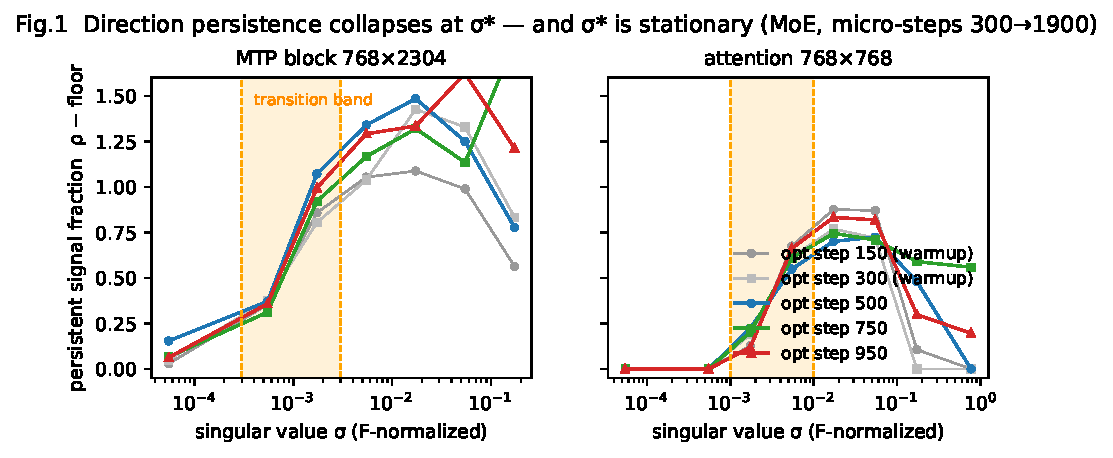
\includegraphics[keepaspectratio,alt={Fig.1: \textbackslash rho(\textbackslash sigma) collapse and stationarity}]{figures/fig1_persistence.pdf}}
\caption{Fig.1: \(\rho(\sigma)\) collapse and stationarity}
\end{figure}

\(\sigma^*\) is \emph{not} monotone in matrix size or aspect ratio: the
within-MoE variation (30\(\times\)) is as large as the
cross-architecture shift (§5.4). \(\sigma^*\) must be measured per shape
group; it is neither a universal constant nor an MP formula.

\subsection{\texorpdfstring{4.3 \(\sigma^*\) is stationary, and the
collapse is a band, not a step
(P30)}{4.3 \textbackslash sigma\^{}* is stationary, and the collapse is a band, not a step (P30)}}\label{sigma-is-stationary-and-the-collapse-is-a-band-not-a-step-p30}

A natural worry: \(\sigma^*\) measured during warmup may expire later.
Late-run snapshots (optimizer steps 500/750/950 = micro-steps
1000/1500/1900; probe\_p30\_latesnap) show the boundary does not move
--- shown here for the two lowest-\(\sigma^*\) groups, the ones §8 turns
on:

{\def\LTcaptype{none} % do not increment counter
\begin{longtable}[]{@{}lllll@{}}
\toprule\noalign{}
group & \(\sigma\) bin & signal fraction @500 & @750 & @950 \\
\midrule\noalign{}
\endhead
\bottomrule\noalign{}
\endlastfoot
MTP 768\(\times\){}2304 & {[}1e-5, 3e-4) & 0.15 & 0.07 & 0.06 \\
& {[}3e-4, 1e-3) & 0.37 & 0.31 & 0.36 \\
& {[}1e-3, 3e-3) & 1.07 & 0.92 & 1.00 \\
& {[}3e-3, 1e-2) & 1.34 & 1.17 & 1.29 \\
shared FFN 768\(\times\){}1536 & {[}3e-4, 1e-3) & 0.76 & 1.13 &
0.78 \\
& {[}1e-3, 3e-3) & 1.25 & 1.08 & 1.43 \\
\end{longtable}
}

(Fractions are \(\rho\) minus the estimator floor; \(\approx\){}1 =
fully persistent.) Two facts in this table drive everything downstream:
\textbf{(i)} the collapse is sharp in log \(\sigma\), and stationary
across micro-steps 300\(\to\){}1900; \textbf{(ii)} it is \emph{not} a
step --- the signal fraction climbs gradually (\(\approx\){}0.3
\(\to\) 1.0 \(\to\) 1.3) across nearly a decade for the heavy-tailed
groups. We call {[}\(\sigma^*\), \(\sigma^*_{\mathrm{upper}}\){]} the
\textbf{transition band}.

\textbf{Operational band edges} (v3; replaces eyeballing). Bin
per-direction values by log \(\sigma\) (bins {[}1e-5, 3e-4, 1e-3, 3e-3,
1e-2, \ldots{]}, \(\times\)√10); per bin take the \emph{median} \(\rho\)
and \emph{median} floor (the median is essential --- the floor blows up
at tiny \(\sigma\)); excess := median \(\rho\) - median floor.
\(\sigma^*_{\mathrm{upper}}\) := the lower edge of the first bin with
excess \(\geq\) 0.9; \(\sigma^*\) := the lower edge of the first bin
with excess \(\geq\) 0.3. Recomputed over all groups and snapshot steps
(\texttt{experiments/sigma\_upper.py} on the p18 dumps,
\texttt{experiments/sigma\_upper\_from\_txt.py} on the p30 tables):

{\def\LTcaptype{none} % do not increment counter
\begin{longtable}[]{@{}
  >{\raggedright\arraybackslash}p{(\linewidth - 4\tabcolsep) * \real{0.3333}}
  >{\raggedright\arraybackslash}p{(\linewidth - 4\tabcolsep) * \real{0.3333}}
  >{\raggedright\arraybackslash}p{(\linewidth - 4\tabcolsep) * \real{0.3333}}@{}}
\toprule\noalign{}
\begin{minipage}[b]{\linewidth}\raggedright
shape group
\end{minipage} & \begin{minipage}[b]{\linewidth}\raggedright
\(\sigma^*\)
\end{minipage} & \begin{minipage}[b]{\linewidth}\raggedright
\(\sigma^*_{\mathrm{upper}}\) (steps 500/750/950)
\end{minipage} \\
\midrule\noalign{}
\endhead
\bottomrule\noalign{}
\endlastfoot
MTP 768\(\times\){}2304 / 2304\(\times\){}768 & 3e-4--1e-3 & 1e-3 /
1e-3 / 1e-3 --- stationary \\
shared FFN 768\(\times\){}1536 / 1536\(\times\){}768 & 3e-4--1e-3 &
1e-3 / 3e-4 / 1e-3 \\
attention q/k/v 768\(\times\){}768 & 0.001--0.003 & no crossing below
1e-2 (excess 0.70--0.83 in {[}1e-2, 3e-2)) \\
o\_proj 768\(\times\){}384 / 384\(\times\){}768 &
\(\approx\){}0.003 & \(\approx\){}3e-3, noisy at later steps \\
KDA gates 96\(\times\){}768 / 768\(\times\){}96 & 0.001--0.003 & no
crossing \(\leq\) 3e-2 (excess \(\lesssim\) 0.5) \\
routed experts gu/dw & 0.003--0.01 & no crossing \(\leq\) 1e-1 (excess
\(\lesssim\) 0.5) \\
kv\_up 128\(\times\){}768 & no collapse in view & --- \\
\end{longtable}
}

So the band is narrow for the heavy-tailed low-\(\sigma^*\) groups
(upper edge \(\approx\){}1--3\(\times\)\(\sigma^*\)) and wide for
attention and the expert stacks (upper edge ≳10\(\times\)\(\sigma^*\);
for the routed experts the fraction never reaches 0.9 in view --- the
``band'' there spans the measured spectrum, consistent with their softer
collapse, §4.2). Where a single knee must serve all groups, the binding
constraint is the parameter-dominant attention block, whose upper edge
is \(\approx\){}1e-2.

\subsection{4.4 The measurement doubles as a diagnostic: a silent
training
bug}\label{the-measurement-doubles-as-a-diagnostic-a-silent-training-bug}

The step-150/300 snapshots showed 20/20 sampled gate\_down matrices with
identically zero gradient --- impossible unless something upstream is
pinned. Cause: hyperball pinning projects every update back to the
pre-update Frobenius norm, so a zero-initialized matrix is pinned at
radius 0 \emph{forever}. GatedNorm.gate\_up (zero-init by design) had
therefore been frozen in every historical run, the gate stayed at
identity, and gate\_down received no gradient. Fix: gate\_up moved to
the AdamW group (standard ``zero-init gates go to Adam'' practice) plus
a zero-norm guard in the projection; regression test
\texttt{test\_muonh\_zeroinit.py}. All probe numbers in this paper are
post-fix unless explicitly labeled; the fix shifted the baseline by
\(\approx\){}0.04 nat, so pre-fix and post-fix numbers are never
subtracted across frames.

\section{5. The law}\label{the-law}

\subsection{5.1 Statement}\label{statement}

\textbf{Definitions.} For each shape group: \(\sigma^*\) := the collapse
point of \(\rho(\sigma)\) (§2.3); transition band := {[}\(\sigma^*\),
\(\sigma^*_{\mathrm{upper}}\){]} under the operational thresholds of
§4.3 (first bin with excess \(\geq\) 0.3 / \(\geq\) 0.9); knee50 := the
\(\sigma\) receiving half weight under a given spectral response.

\begin{quote}
\textbf{Persistence-boundary law (corrected form).} Give zero weight
below \(\sigma^*\); inside the transition band, shrink by the measured
signal fraction; flatten above \(\sigma^*_{\mathrm{upper}}\). A
single-knee schedule should place knee50 at the \textbf{upper} edge
\(\sigma^*_{\mathrm{upper}}\) --- not at \(\sigma^*\). Deviations are
penalized on both sides, and the two arms of the resulting U-shaped
quality curve span exactly the band: knees at \(\sigma^*\) hand
30--70\%-noise directions full weight (variance injection); knees past
\(\sigma^*_{\mathrm{upper}}\) under-whiten fully persistent directions.
\end{quote}

The naive reading (binary: zero below \(\sigma^*\), flat above) is what
§8 falsifies; the corrected form is what the intervention data below
supports.

\subsection{5.2 Intervention: the U-curve on the MoE (500-step
tier)}\label{intervention-the-u-curve-on-the-moe-500-step-tier}

Only the knee of the cubic schedule is varied. Since v3 the full U lives
in a single frame (post-fix; the pre-fix frame is retained only for the
qualitative extremal points marked †). Paired, same seed (1337),
baseline b05 = 5.264, paired noise floor \(\pm\){}0.05:

{\def\LTcaptype{none} % do not increment counter
\begin{longtable}[]{@{}
  >{\raggedright\arraybackslash}p{(\linewidth - 8\tabcolsep) * \real{0.2000}}
  >{\raggedright\arraybackslash}p{(\linewidth - 8\tabcolsep) * \real{0.2000}}
  >{\raggedright\arraybackslash}p{(\linewidth - 8\tabcolsep) * \real{0.2000}}
  >{\raggedright\arraybackslash}p{(\linewidth - 8\tabcolsep) * \real{0.2000}}
  >{\raggedright\arraybackslash}p{(\linewidth - 8\tabcolsep) * \real{0.2000}}@{}}
\toprule\noalign{}
\begin{minipage}[b]{\linewidth}\raggedright
probe
\end{minipage} & \begin{minipage}[b]{\linewidth}\raggedright
knee50
\end{minipage} & \begin{minipage}[b]{\linewidth}\raggedright
loss@500
\end{minipage} & \begin{minipage}[b]{\linewidth}\raggedright
\(\Delta\) vs b05
\end{minipage} & \begin{minipage}[b]{\linewidth}\raggedright
reading
\end{minipage} \\
\midrule\noalign{}
\endhead
\bottomrule\noalign{}
\endlastfoot
classic NS5 (P31) & \(\approx\){}0.001 & 5.358 & \textbf{+0.094} & far
left arm \\
cubic5b002 (7 steps, P20) & \(\approx\){}5e-4 (at \(\sigma^*\)) &
5.318 & \textbf{+0.054} & left arm: transition band at full weight \\
cubic5 (P32) & \(\approx\){}0.004 & 5.274 & +0.010 & left shoulder \\
\textbf{cubic5b05 (default, P19)} & \(\approx\){}0.010
(\(\approx\)\(\sigma^*_{\mathrm{upper}}\)) & \textbf{5.264} & --- &
\textbf{peak} \\
cubic5b10 (P33) & \(\approx\){}0.02 & 5.349 & \textbf{+0.085} & right
arm \\
PE5 (sharp knee) †pre-fix & \(\lesssim\){}0.001 & +0.14 vs.~classic &
& far left; sharper is worse \\
no-NS (norm only) †pre-fix & none & +0.34 vs.~classic & & no whitening
at all \\
frac family (no flat top) †pre-fix & --- & +0.20\ldots0.28 & & respects
the knee but never flattens --- right-arm failure by construction \\
\end{longtable}
}

\textbf{Seeds.} The peak and both arms now have 3 seeds each (P25,
P36--P39). Per-seed \(\Delta\) vs.~b05 --- b002: +0.054 / +0.014 /
+0.024 (seeds 1337/1338/1339); b10: +0.085 / +0.065 / +0.038. The arm
penalties are positive on \textbf{every} seed; cross-seed \(\sigma\) of
the \(\Delta\) is \(\approx\){}0.02 nat for both arms. The monotone
trio \(\tau\)(1e-3) = 0.86 / 0.47 / 0.12 \(\to\) +0.14 / 0 / -0.08 (PE5
/ classic / cubic5) was the original smoking gun.

\textbf{Arms = band width.} Left arm: a knee at \(\sigma^*\) \(\approx\)
5e-4 hands the band {[}\(\sigma^*\), \(\approx\){}3e-3{]} --- measured
30--70\% non-persistent for the heavy-tailed groups --- full weight.
Right arm: a knee at 0.02 \textgreater{} \(\sigma^*_{\mathrm{upper}}\)
under-whitens the range {[}3e-3, 1e-2{]} whose measured signal fraction
is \(\approx\){}1. The peak sits between, at the upper edge of the
parameter-dominant attention band (§4.3). This is the measurable version
of \(t^*\)'s shape intuition.

\begin{figure}
\centering
\pandocbounded{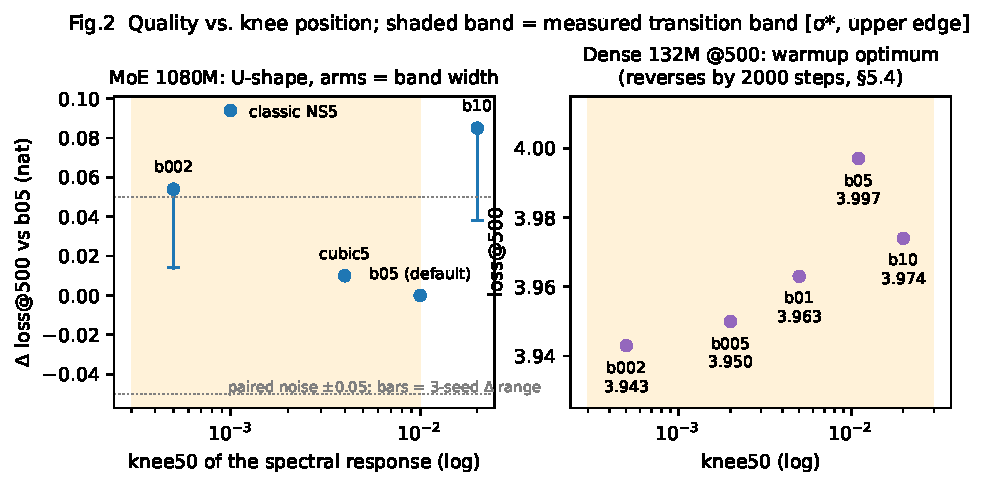
\includegraphics[keepaspectratio,alt={Fig.2: U-curve on two architectures}]{figures/fig2_ucurve.pdf}}
\caption{Fig.2: U-curve on two architectures}
\end{figure}

\subsection{5.3 Prediction scorecard (pre-registered in the theory
note)}\label{prediction-scorecard-pre-registered-in-the-theory-note}

{\def\LTcaptype{none} % do not increment counter
\begin{longtable}[]{@{}
  >{\raggedright\arraybackslash}p{(\linewidth - 4\tabcolsep) * \real{0.3333}}
  >{\raggedright\arraybackslash}p{(\linewidth - 4\tabcolsep) * \real{0.3333}}
  >{\raggedright\arraybackslash}p{(\linewidth - 4\tabcolsep) * \real{0.3333}}@{}}
\toprule\noalign{}
\begin{minipage}[b]{\linewidth}\raggedright
\#
\end{minipage} & \begin{minipage}[b]{\linewidth}\raggedright
prediction
\end{minipage} & \begin{minipage}[b]{\linewidth}\raggedright
verdict
\end{minipage} \\
\midrule\noalign{}
\endhead
\bottomrule\noalign{}
\endlastfoot
1 & optimal knee \(\approx\) \(\lambda_+\) closed form; raising the knee
helps up to \(\lambda_+\) & \textbf{half}: raising helps up to b05 then
U-turns (b10 +0.09) \(\checkmark\); the closed-form calibration fails
(§4.1) \(\times\) --- replaced by measured \(\sigma^*\) \\
2 & direction correlation collapses at \(\hat{\lambda}_+\) &
\textbf{form right, position corrected}: \(\rho(\sigma)\) collapses
(sharper than predicted), but at \(\sigma^*\) \(\neq\)
\(\hat{\lambda}_+\) \\
3 & per-shape knee scales as (1/\(\sqrt{m}\) + 1/\(\sqrt{n}\)) &
\textbf{not confirmed}: measured \(\sigma^*\) does not follow MP ratios
(§4.2); per-head compensation is unnecessary post-fix (§6) \\
4 & knee scales as \(\sqrt{B}\) with batch size & \textbf{not confirmed}
at B/2 (P22): b07 vs.~b05 within noise; the lever may be ESS-dominated
at fixed \(\beta\) \\
5 & residual headroom below the current knee region & \textbf{direction
right}: both arms harmful, interior peak (P17/P20) --- U confirmed \\
\end{longtable}
}

Zero of two quantitative scaling laws survived; the entire qualitative
frame (U-shape, knee = persistence boundary, zero weight below
\(\sigma^*\)) did. Hence the paper's form: a
measurement-plus-intervention law rather than a closed-form prediction.

\subsection{5.4 Externalization: the law replicates on a dense model ---
by
moving}\label{externalization-the-law-replicates-on-a-dense-model-by-moving}

Dense 132M platform, same protocol, 500-step tier, seed 1337 (paired
floor \(\pm\){}0.05; five-point knee grid, all in the post-fix frame):

{\def\LTcaptype{none} % do not increment counter
\begin{longtable}[]{@{}
  >{\raggedright\arraybackslash}p{(\linewidth - 6\tabcolsep) * \real{0.2500}}
  >{\raggedright\arraybackslash}p{(\linewidth - 6\tabcolsep) * \real{0.2500}}
  >{\raggedright\arraybackslash}p{(\linewidth - 6\tabcolsep) * \real{0.2500}}
  >{\raggedright\arraybackslash}p{(\linewidth - 6\tabcolsep) * \real{0.2500}}@{}}
\toprule\noalign{}
\begin{minipage}[b]{\linewidth}\raggedright
schedule
\end{minipage} & \begin{minipage}[b]{\linewidth}\raggedright
knee50
\end{minipage} & \begin{minipage}[b]{\linewidth}\raggedright
loss@500
\end{minipage} & \begin{minipage}[b]{\linewidth}\raggedright
reading
\end{minipage} \\
\midrule\noalign{}
\endhead
\bottomrule\noalign{}
\endlastfoot
b002 (P26c) & \(\approx\){}5e-4 & \textbf{3.943} & knee at the dense
\(\sigma^*\) --- plateau edge \\
b005 (P35) & \(\approx\){}2e-3 & 3.950 & plateau \\
b01 (P34) & \(\approx\){}5e-3 & 3.963 & plateau, drifting up \\
b10 (P26b) & \(\approx\){}0.02 & 3.974 & under-whitening cost
visible \\
b05 (P26a) & \(\approx\){}0.011 & 3.997 & \textbf{worst at this
tier} \\
\end{longtable}
}

The MoE ranking does \textbf{not} transfer at this tier: the MoE optimum
b05 is \emph{worst} here, and the best point sits at b002 (vs.~b05:
-0.054, beyond the paired floor). The three lowest knees (b002/b005/b01)
span 0.020 nat --- a plateau within the noise floor, i.e.~the dense left
arm has not yet appeared even with the knee at \(\sigma^*\) itself.
Measurement explains the shift before any curve-fitting
(probe\_p27\_dense\_snap): dense \(\sigma^*\) \(\approx\) 3e-4--1e-3
(attention), \(\leq\){}0.003 (FFN) --- an order of magnitude
\emph{below} the MoE's 0.003--0.01. What does \textbf{not} move is the
band's upper region: under the §4.3 rule the dense FFN's excess reaches
0.9 only at \(\approx\){}3e-2 and the dense attention block never
crosses 0.9 in view (0.5--0.87 across {[}3e-3, 3e-1)) --- the dense band
is \emph{wide}, overlapping the MoE's 1e-2--3e-2 region. So what the
10\(\times\) shift moves is the band's \textbf{lower} edge.

\textbf{The 2000-step tier reverses the ranking --- and explains it}
(P40--P42, paired, seed 1337, loss@1900). b05 completes cleanly at
\textbf{2.905}. b005 completes at 2.977 --- \textbf{+0.072 worse than
b05}, beyond the paired floor. b002, the 500-step winner, first
\emph{replicates} its advantage at step 500 of the same run (3.929
vs.~b05's 3.994, -0.065, matching the 500-step tier's -0.054), then
spikes to 8.36 at step \(\approx\){}600, half-recovers, and is
irreversibly NaN by step \(\approx\){}1000 (the NaN guard skips
non-finite updates but cannot un-poison the parameters). The paired b05
control passes the \emph{identical} data order without any excursion, so
the divergence is a property of the schedule, not the data.

Read through §7's mechanism, this is the predicted asymmetry between the
two arms' costs. Under-whitening (right arm) is a per-step efficiency
loss: paid immediately, absorbable by the learning rate --- hence
visible already at 500 steps, where b05 pays it. Injecting
non-persistent directions (left arm) is variance that \emph{compounds}
in the momentum state: nearly free at 500 steps (the plateau reaches all
the way down to \(\sigma^*\)), decisive by 2000 (b005 concedes 0.07;
b002 destabilizes outright). The warmup tier therefore biases knee
selection \textbf{downward}, and the steady-state optimum sits higher
--- on dense at knee50 \(\approx\) 0.01, the same value as the MoE
default, inside the wide measured band.

The MoE's right arm shows the same asymmetry in mirror image: b10's
warmup penalty (+0.082 at step 500 of the 2000-step run, replicating the
500-step tier's +0.085) fully closes by step 1000 and ends nominally
\emph{ahead} at -0.018 at step 1900 --- within the paired floor (P43
vs.~the P28a baseline 4.087; component split main -0.036 / MTP +0.058).
Under-whitening fades; injection compounds. The MoE default b05 is
therefore no longer \emph{better} than b10 at 2000 steps, but it is not
worse either --- the default survives, now on 2000-step evidence rather
than warmup evidence.

The §8 lesson --- warmup optima are not steady-state optima --- thus
applies to the headline grid itself, and the law's practical form
hardens: \textbf{place knee50 at the band's upper edge, never at
\(\sigma\)*}. (Single seed and one run per point at this tier; the b002
divergence is one event, §10.)

\section{6. Scaling and robustness
checks}\label{scaling-and-robustness-checks}

\begin{figure}
\centering
\pandocbounded{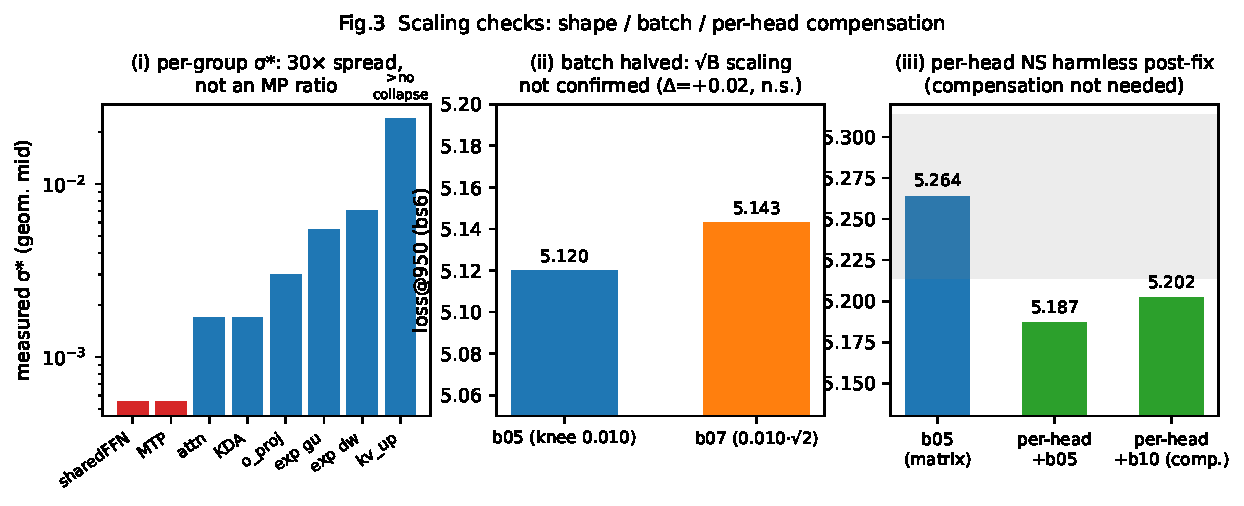
\includegraphics[keepaspectratio,alt={Fig.3: shape / batch / per-head}]{figures/fig3_scaling.pdf}}
\caption{Fig.3: shape / batch / per-head}
\end{figure}

\begin{itemize}
\tightlist
\item
  \textbf{Shape axis} (scorecard row 3). Per-head NS
  (64\(\times\){}768 blocks instead of 768\(\times\){}768) with
  MP-motivated knee compensation \(\times\){}1.9 (P21: 5.202, -0.06)
  and without (P21b: 5.187, -0.08) are both fine at 500 steps ---
  uncompensated slightly better. The pre-fix stack had per-head at +0.14
  harmful; this does not reproduce post-fix and is attributed to
  interactions in the old (gate-frozen) stack. The strong MP-ratio form
  of shape scaling is not supported; per-group \(\sigma^*\) measurement
  is the operative replacement.
\item
  \textbf{Batch axis.} Halving the effective batch (bs6 \(\times\)
  accum2), b07 (= b05\(\cdot\)\(\sqrt{2}\)) is not better than b05
  (+0.02, within noise; P22). The \(\sqrt{B}\) prediction is unconfirmed
  at B/2; at fixed \(\beta\) the noise level may be ESS-dominated rather
  than batch-dominated.
\item
  \textbf{Seeds.} Cross-seed \(\sigma\) of absolute loss = 0.11 nat
  (P25); cross-seed \(\sigma\) of the \emph{paired} arm-vs-peak
  \(\Delta\) is \(\approx\){}0.02 nat, and both arm penalties are
  positive on all three seeds (§5.2). All \(\leq\){}0.09-nat claims at
  the 500-step tier are \emph{paired} claims (\(\pm\){}0.05 floor); we
  claim the U's direction, not exact nat values, across seeds. The
  2000-step effects in §8 (+0.18 total, +0.47 on the MTP component)
  exceed both floors.
\end{itemize}

\section{7. A zero-parameter unification of failure
modes}\label{a-zero-parameter-unification-of-failure-modes}

One mechanism, no fitted constants: \textbf{weight given to zero-overlap
(non-persistent) directions is pure variance injection --- first-order
harmful; bandwidth variation among persistent directions is absorbed by
the learning rate --- second-order harmless.} The measured \(\sigma^*\)
table (§4.2) turns this into per-case arithmetic:

{\def\LTcaptype{none} % do not increment counter
\begin{longtable}[]{@{}
  >{\raggedright\arraybackslash}p{(\linewidth - 2\tabcolsep) * \real{0.5000}}
  >{\raggedright\arraybackslash}p{(\linewidth - 2\tabcolsep) * \real{0.5000}}@{}}
\toprule\noalign{}
\begin{minipage}[b]{\linewidth}\raggedright
observation
\end{minipage} & \begin{minipage}[b]{\linewidth}\raggedright
account
\end{minipage} \\
\midrule\noalign{}
\endhead
\bottomrule\noalign{}
\endlastfoot
PE5 +0.14 (\(\tau\)(1e-3) = 0.86) & \(\sigma\) = 1e-3 is below every
measured attention boundary: a non-persistent direction at 0.86 weight
--- maximal injection \\
classic NS5 (\(\tau\)(1e-3) = 0.47) & the same direction at half weight
--- between PE5 and cubic5, as observed \\
cubic5 -0.08 (\(\tau\)(1e-3) = 0.12) & least injection of the trio;
three points monotone in the predicted direction \\
no-NS, norm-only +0.34 & \(\tau\) \(\propto\) \(\sigma\): top directions
monopolize the step; mid-strength \emph{persistent} directions
underweighted --- the opposite failure (under-whitening) \\
stale polar factor +0.4\ldots0.5, worst in warmup & full weight on
directions that have \emph{rotated away} --- zero-overlap full weight in
the extreme; momentum rotates fastest in warmup \(\Rightarrow\) maximal
harm there \(\checkmark\) \\
per-head NS +0.14 (pre-fix stack only) & cutting to 64\(\times\){}768
raises the block's noise edge \(\approx\){}1.8\(\times\) (MP
estimate), doubling injected noise mass at fixed coefficients. Not
reproduced post-fix (§6) --- consistent, not confirmed. Also matches
Pion's report that per-head helps only combined with a high-pass \\
Pion's RLVR gains & low-SNR regimes raise the boundary; a fixed classic
knee is then \emph{relatively} too low --- tail suppression is the
predicted fix. Consistent with Pion's gains appearing in RLVR/VLA, not
pretraining \\
\end{longtable}
}

Zero-parameter does not mean unfalsifiable: this account predicted the
U's left arm before it was measured (P20), predicted the dense-model
reversal at the warmup tier (§5.2\(\to\)§5.4), and predicted the
localization of EdgeCubic's failure (§8). Its sharpest implication ---
injection compounds, under-whitening does not --- is what the 2000-step
dense re-reversal observes (§5.4).

\section{8. Method attempt and controlled negative result:
EdgeCubic}\label{method-attempt-and-controlled-negative-result-edgecubic}

\begin{figure}
\centering
\pandocbounded{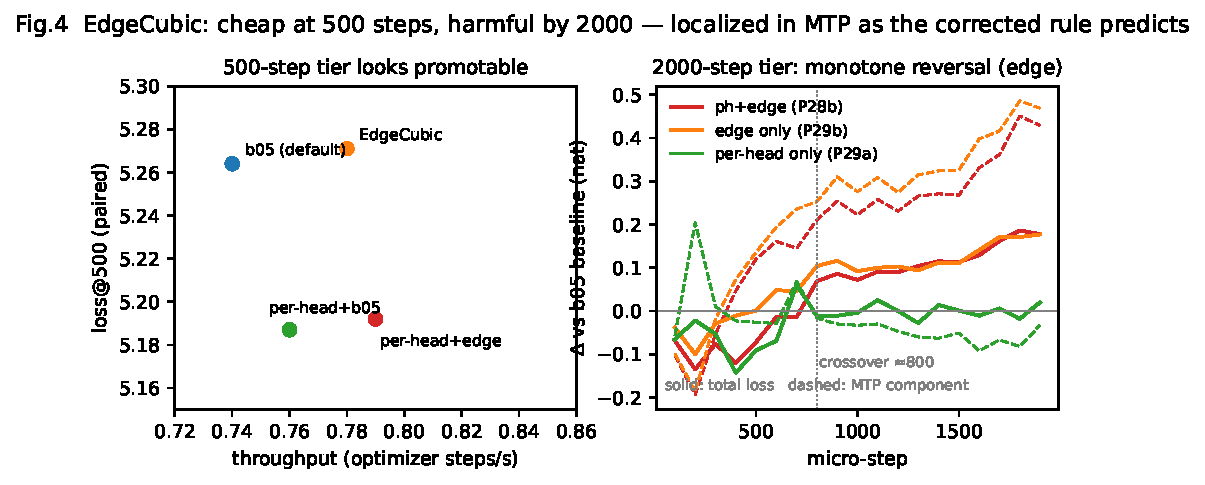
\includegraphics[keepaspectratio,alt={Fig.4: Pareto + 2000-step reversal}]{figures/fig4_pareto_reversal.pdf}}
\caption{Fig.4: Pareto + 2000-step reversal}
\end{figure}

The naive engineering reading --- set each shape group's knee at its
measured \(\sigma^*\) (l0 = 4.5\(\sigma^*\), so knee50 \(\approx\)
\(\sigma^*\)), let the schedule generator pick its own step count (4--8
steps; fewer GEMMs at higher knees) --- is a coefficient-table swap
(\texttt{VIBY\_MUONH\_EDGE=1}).

\begin{itemize}
\tightlist
\item
  \textbf{500-step tier}: quality-neutral (5.271 vs.~5.264, within the
  paired floor) at \textbf{+5.4\% throughput} (0.78 vs.~0.74 step/s;
  0.79 with per-head). Passed the pre-registered promotion bar.
\item
  \textbf{2000-step tier}: monotone reversal. \(\Delta\){}loss crosses
  zero at step \(\approx\){}800 and grows to \textbf{+0.18 at step
  1900}, with 4/5 of the regression in the auxiliary MTP loss
  (\textbf{+0.47}, vs.~+0.05 main).
\item
  \textbf{Single-variable attribution} (2000 steps, same seed): per-head
  alone is neutral throughout (\textbar{}\(\Delta\)\textbar{} \(\leq\)
  0.09; MTP slightly better, -0.03\ldots-0.09); EdgeCubic alone
  reproduces the full regression (+0.18 / +0.04 / +0.47) --- additive,
  no interaction. The damage is localized in the MTP/shared-FFN groups
  --- exactly the groups that received the lowest knee (l0 = 0.0025).
\item
  \textbf{Mechanism discrimination} (P30, §4.3): \(\sigma^*\) did not
  drift, so staleness is not the cause; the binary rule is. The
  lowest-knee groups have the widest transition bands (heaviest tails,
  Zipf \(\approx\) -2.4): ``flatten to 1 above \(\sigma^*\)'' hands a
  near-decade of 30--70\%-noise directions full weight. The harm
  accumulates slowly and is invisible at 500 steps --- the
  warmup-vs-steady-state lesson of stale-D, re-learned at the method
  level. (And re-learned a third time at the grid level: the dense
  500-step knee plateau reverses by 2000 steps, §5.4.)
\end{itemize}

We retain \textbf{cubic5b05 as the default} and archive EdgeCubic behind
its env flag. The corrected law suggests two rescues --- knees at the
\emph{upper} band edge (which for these groups is \(\approx\){}b05's
position: the status quo), or per-group signal-fraction shrinkage (which
is \(t^*\) itself, realized from measurements rather than a model) ---
but any variant must re-pass the dual-duration gate; we deliberately do
not promote one here.

\textbf{Why the negative result strengthens the law}: the binary rule
fails exactly where the corrected law says it must (lowest \(\sigma^*\),
widest band, most sensitive block), with an effect size (+0.47 on the
component loss) that dwarfs both noise floors. A law that calls its own
naive misreading's failure mode, in advance and in the right location,
is doing work.

\section{9. Related work}\label{related-work}

\begin{itemize}
\tightlist
\item
  \textbf{Spectral shaping in Muon}: classic NS5 (Jordan et al.); Polar
  Express (sharp quintic); ``How Much Orthogonalization Does Muon
  Need?'' (arXiv 2606.00371) --- source of the relaxed-cubic family and
  the non-monotonicity observation this paper explains; Muon-p (arXiv
  2606.13867) --- impossibility theorem, compatible with \(t^*\) (§3.3);
  Pion (arXiv 2605.19282) --- promotion/suppression split; tail
  suppression \(\approx\) a high knee (our left arm), and their RLVR
  observation is the low-SNR limit of our law (§7).
\item
  \textbf{Outside the equivariant/stateless class}: NorMuon (arXiv
  2510.05491; in our frame, row-wise second moments are the first step
  of anisotropic-noise whitening --- §4.1 measured exactly that
  anisotropy), Aurora (arXiv 2606.27715), RowFloor, per-head reshaping
  (equivariance breaking); SOAP/Shampoo, Dion's error feedback (state);
  Mousse (arXiv 2603.09697; curvature). The \(\sigma^*\) measurement is
  orthogonal to and composable with all of these.
\item
  \textbf{Heavy-tailed training spectra}: HT-SR-style heavy tails are
  documented for weights/Hessians; we find momentum spectra are smooth
  heavy-tailed too --- precisely what breaks MP calibration and widens
  the transition band.
\item
  \textbf{RMT toolbox}: Marchenko--Pastur (1967); BBP; Benaych-Georges
  \& Nadakuditi (2012) overlap formulas (validated synthetically at
  2\%); Gavish \& Donoho (2017) optimal shrinkage (different objective
  --- §3.3); von Neumann (1937) representation behind §3.1.
\item
  \textbf{Optimizer-benchmark evidence}: the nanoGPT optimizer track's
  decomposable gain stack (Muon \(\to\) Muon\(^2\) \(\to\) NorMuonH
  \(\to\) u/w-floor \(\to\) radial brake \(\to\) RowFloor + cautious WD;
  3600 \(\to\) 2690 steps) corroborates that optimizer progress composes
  from mechanism-level fixes; this paper contributes a measurable law
  for one core mechanism in that stack.
\end{itemize}

\section{10. Limitations and honest
boundaries}\label{limitations-and-honest-boundaries}

\begin{itemize}
\tightlist
\item
  \textbf{Scale and window.} All probes \(\leq\){}2000 micro-steps,
  132M/1080M models, one codebase, single node, bf16. Stationarity of
  \(\sigma^*\) is established for micro-steps 300--1900 only; behavior
  at 100k+ steps, other \(\beta\), and much larger batches is unknown.
  The \(\sqrt{B}\) law failing at B/2 does not bound B/8.
\item
  \textbf{Frames.} The gate-fix of P19 moved all absolute losses
  (\textasciitilde0.04 nat); the full five-point MoE U and the
  five-point dense grid both live entirely in the post-fix frame (§5.2,
  §5.4). Pre-fix points survive only as qualitative extremal markers (†)
  and cross-frame \(\Delta\){}s are never taken.
\item
  \textbf{Seeds.} Peak and both arms have 3 seeds each; per-seed arm
  penalties are uniformly positive (§5.2). Interior points near the peak
  (cubic5) and the dense grid remain single-seed paired comparisons. The
  2000-step tier (dense P40--P42, MoE P43-vs-P28a) is single-seed, one
  run per point; the b002 divergence is a single event --- its
  schedule-specificity, not its exact probability, is what the paired
  control establishes.
\item
  \textbf{Estimator.} The i.i.d. reading of the \(\rho\) chance floor is
  approximate under the measured anisotropy; a row/column-whitened
  variant (NorMuon-style preprocessing) is the principled next step and
  may sharpen \(\sigma^*\).
\item
  \textbf{Objective proxy.} The theory optimizes per-step E{[}descent{]}
  - variance, not full training dynamics; all verdicts here are
  empirical.
\item
  \textbf{Unmeasured region.} kv\_up 128\(\times\){}768 shows no
  collapse in view (\(\rho\) \textgreater{} 1 at \(\sigma_{\min}\) =
  0.024); the law is silent there beyond ``flatten''. Dense-band upper
  edges are early-window measurements (optimizer steps 150/300); their
  late-window stationarity is assumed from the MoE (P30), not
  re-measured.
\item
  \textbf{Open mechanism.} The 10\(\times\) dense-vs-MoE shift of the
  band's \emph{lower} edge is measured, not explained; the upper region
  (\(\approx\){}1e-2--3e-2, excess never quite reaching 0.9 for
  attention) is common to both architectures, and why the steady-state
  optimum lands at knee50 \(\approx\) 0.01 on both is consistent with,
  not derived from, the band picture.
\end{itemize}

\section{11. Conclusion}\label{conclusion}

The whitening knee of Muon-style optimization is governed by a
measurable persistence boundary \(\sigma^*\) and its transition band.
The boundary is read off cross-microbatch correlations with no
distributional assumptions, is stationary in our training window,
predicts the quality optimum across two architectures (five-point knee
grids on each, three seeds on the MoE arms and peak), and explains six
known failure modes plus one literature observation in one stroke. Its
naive binary reading fails in a way the refined law predicts --- the
U-curve's arms \emph{are} the transition band --- and the arms' costs
are temporally asymmetric: under-whitening is paid upfront, variance
injection compounds until, at 2000 steps, it can destabilize training
outright. Practically: measure \(\rho(\sigma)\) before touching the
knee; place the half-weight point at the band's upper edge; and distrust
500-step promotion gates --- warmup optima are not steady-state optima,
on both the method level (§8) and the grid level (§5.4). The closed-form
RMT knee failed; the measured knee stands.

\section{References (informal; expanded in research/SPECTRAL\_THEORY.md
§9 and research/OPTIMIZER\_RESEARCH.md
§1.3)}\label{references-informal-expanded-in-researchspectral_theory.md-9-and-researchoptimizer_research.md-1.3}

\begin{enumerate}
\def\labelenumi{\arabic{enumi}.}
\tightlist
\item
  Jordan et al.~--- Muon. 2. Bernstein \& Newhouse --- Old optimizer,
  new norm.
\item
  Polar Express (arXiv 2505.16932). 4. How Much Orthogonalization Does
  Muon Need? (arXiv 2606.00371). 5. Pion (arXiv 2605.19282). 6. NorMuon
  (arXiv 2510.05491). 7. Aurora (arXiv 2606.27715). 8. Mousse (arXiv
  2603.09697). 9. Muon-p (arXiv 2606.13867). 10. Shampoo; SOAP; Dion
  (arXiv 2504.05295). 11. Marchenko \& Pastur (1967). 12.
  Benaych-Georges \& Nadakuditi (2012). 13. Gavish \& Donoho (2017). 14.
  von Neumann (1937).
\end{enumerate}

\section{Appendix A. Protocol and
reproducibility}\label{appendix-a.-protocol-and-reproducibility}

\begin{itemize}
\tightlist
\item
  All probes: seed 1337, paired data order; screening 500 micro-steps,
  confirmation 2000 micro-steps, log every 100; one training job at a
  time.
\item
  Probe \(\to\) artifact map: P13 cubic5 \(\cdot\) P14/15 frac family
  \(\cdot\) P16 b05 \(\cdot\) P17 b10 \(\cdot\) P18 snapshots (optimizer
  steps 150/300) \(\cdot\) P19 gate-fix baseline \(\cdot\) P20 b002
  \(\cdot\) P21/P21b per-head \(\pm\) compensation \(\cdot\) P22
  batch-half \(\cdot\) P23 EdgeCubic \(\cdot\) P24 per-head+edge
  \(\cdot\) P25 seeds \(\cdot\) P26 dense knees (a: b05, b: b10, c:
  b002) \(\cdot\) P27 dense snapshots \(\cdot\) P28 2000-step
  confirmation (a: baseline, b: per-head+edge) \(\cdot\) P29
  single-variable attribution (a: per-head, b: edge) \(\cdot\) P30 late
  snapshots (optimizer steps 500/750/950) \(\cdot\) P31--P33 post-fix U
  re-runs (classic / cubic5 / b10) \(\cdot\) P34/P35 dense b01/b005
  \(\cdot\) P36--P39 arm seeds (b002/b10 \(\times\) 1338/1339) \(\cdot\)
  P40--P42 dense 2000-step tier (b002 diverged / b05 / b005) \(\cdot\)
  P43 MoE b10 2000-step check (vs.~P28a). Logs in
  \texttt{research\_runs/probe\_*/console.log}; analysis dumps in
  \texttt{probe\_p18\_snap}, \texttt{probe\_p27\_dense\_snap},
  \texttt{probe\_p30\_latesnap} (+ \texttt{mpfit\_all.txt},
  \texttt{sigma\_upper.txt}); queue ledger
  \texttt{research\_runs/gap\_queue\_status.tsv},
  \texttt{research\_runs/dense\_2k\_status.tsv}.
\item
  Code: \texttt{trainer/muon.py} (schedules \texttt{\_CUBIC5B*\_COEFFS},
  \texttt{\_cubic\_schedule}, \texttt{\_EDGE\_L0\_*}),
  \texttt{trainer/snapshot.py}, \texttt{experiments/mp\_fit.py}
  (synthetic validation included), \texttt{experiments/sigma\_upper*.py}
  (operational band edge, §4.3), \texttt{test\_muonh\_zeroinit.py} (§4.4
  regression). The \(\rho(\sigma)\) measurement is also packaged as a
  standalone numpy-only tool, \texttt{kneescope} (companion repository;
  MIT), with synthetic-validation tests.
\item
  Convention: snapshot steps count optimizer updates (2 micro-steps each
  at accumulation 2). A unit mix-up cost one aborted run during P30; the
  convention is now asserted in the tooling docstring.
\end{itemize}

\section{Appendix B. Figures}\label{appendix-b.-figures}

All figures render from repository artifacts:
\texttt{research/figures/fig\{1..4\}\_*.\{png,pdf\}}. Regenerate with
\texttt{uv\ run\ -\/-no-project\ -\/-with\ matplotlib\ python\ experiments/paper\_figs.py}
(parsers read the probe logs and mp\_fit outputs directly).

\begin{itemize}
\tightlist
\item
  \textbf{Fig.1} (existence + stationarity): \(\rho(\sigma)\) per shape
  group, log \(\sigma\); curves for optimizer steps 150/300 (warmup) and
  500/750/950 overlaid; shaded transition band. Data:
  probe\_p18\_snap/mp\_fit\_v2.txt, probe\_p30\_latesnap/mpfit\_all.txt.
\item
  \textbf{Fig.2} (money): left --- MoE \(\Delta\){}loss@500
  vs.~knee50, five post-fix points solid (single frame), pre-fix points
  hollow (qualitative only), shaded transition band, 3-seed \(\Delta\)
  error bars on the two arms; right --- dense 132M five-point grid at
  the 500-step tier with its measured band (\(\sigma^*\) 10\(\times\)
  lower, upper region \(\approx\){}3e-2 shared with the MoE). Data:
  §5.2/§5.4 tables.
\item
  \textbf{Fig.3} (scaling triple): per-group \(\sigma^*\) (log bars);
  batch-half pair; per-head \(\pm\) compensation. Data: §4.2 table, P22,
  P21/P21b.
\item
  \textbf{Fig.4} (Pareto + reversal): 500-step loss vs.~step/s for b05 /
  EdgeCubic / per-head+\{b05, edge\}; 2000-step \(\Delta\){}loss
  (solid) and \(\Delta\){}MTP (dashed) trajectories vs.~the b05
  baseline for ph+edge / edge / per-head. Data: P28/P29 console logs;
  P19/P23/P24 step/s.
\end{itemize}

\end{document}
